\subsection{Архитектура приложения}


\subsubsection{Фреймворк Yii}
\label{section:yii}
Для программной реализации приложения был выбран фреймворк Yii\cite{yii}, написанный на языке
программирования PHP. Он реализован в соответствии с паттерном проектирования MVC\cite{gamma},
предполагая разделение на различные компоненты следующих частей приложения:
\begin{itemize}
\item{
Части, составляющие модель данных
}
\item{
Части, отвечающие за взаимодействиее системы и пользователя
}
\item{ 
Часть, связанная с пользовательским интерфейсом
}
\end{itemize}

Yii унаследовал многие достоинства других фреймворков для PHP, таких как Symfony или Zend, 
при этом обладая многими преимуществами по сравнению с ними, такими как высокая производительность,
удачные архитектурные решения для использования Ajax в совокупности с jQuery и т.д.

\paragraph{Жизненный цикл запроса}
Yii реализует одно из типичных решений для обработке HTTP-запросов пользоваеля, описанные в \cite{fowler}:
FrontContoller (на рис. \ref{gr:yiirequestflow} YiiApp) получает данные запроса, затем на основе
адреса запроса и конфигурации маршрутов выбирает подходящий Controller и action, который формирует текст ответа пользователю.

В отличие от классического Контроллера страниц, в Yii в одном классе принято описывать правила обработки сразу нескольких
типов запросов, каждый в отдельном методе с префиксом ``action'', один из которых в рамках запроса будет вызван
с использованием методов интроспекции из YiiApp.

При генерации HTML-кода ответа в Yii имеет место ``Представление по шаблону'', 
причем весь код страницы делиться на два шаблона: содержание 
для конкретного запроса и ``Layout'', в котором расположены элементы, присутствующие на 
каждой странице.

\begin{figure}[!ht]
\begin{center}
\includegraphics[scale=0.6, trim=0mm 100mm 40mm 0mm, clip]{../resources/uml/YiiRequestFlow.pdf}
\caption{Cхематичная диаграмма взаимодействия, демонстрирующая жизненный цикл пользовательского запроса в Yii}
\label{gr:yiirequestflow}
\end{center}
\end{figure} 

\paragraph{Архитектура фреймворка}
Все компоненты фреймворка разбиты на пакеты-слои, такие как: Контроллеры, Модели, Формы, 
Элементы представления. Причем для каждого слоя выделен отдельный базовый класс ---
 Layer Supertype\cite{fowler}. Кроме того определен базовый класс CComponent, от которого
унаследованы все супертипы слоев, в котором реализована работа с событиями.

Классы-формы используются как посредники между представлениями и моделями, пользователю
они доступны как обычная форма для ввода данных, после отправки которой обновленные данные
из запроса отображаются в поля объекта-модели.

При разработке приложения программисту доступен для использования глобальный объект-реестр,
с помощью которого можно получить доступ ко всем остальным глобальным объектам или сервисам.
Получение самого реестра реализована с применением типового решения Singleton\cite{gamma}.
Кроме всего прочего фреймворк предоставляет возможность разработчику самому добавлять в реестр
объекты-сервисы, которые должны быть доступны из любой точки приложения. 

\paragraph{Работа с БД}Встроенная ORM реализует паттерн проектирования Active Record\cite{fowler},
инкапсулируя работу с базой данных, при взаимодействии с объектами модели предметной области.

Кроме того для классов-моделей предлагаются удобные интерфейсы для определения правил проверки
корректности данных и задания названий полей с учетом мультиязычного интерфейса.

С помощью дополнительного расширения Giix\cite{giix} становится возможной генерация классов модели предметной
области на основе текущей структуры базы данных, причем:
\begin{enumerate}
\item{
  Для каждой таблицы(кроме используемых для реализации связи N:M) генерируется по два класса-модели:
  основной, который предназначен для дальнейшего изменения пользователем, и родительский класс 
  с префиксом ``Base'', в котором описывается логика отображения данных, и который может быть
  сгенерирован заново при изменении структуры таблицы. Также в базовом классе добавляются
  стандартные проверки корректности данных модели, такие как проверки, что формат значений полей объекта
  класса удовлетворяет формату типа соответствующего поля БД (например целое число или дата).
}
\item{
  На основе списка внешних ключей таблиц генерируются правила отображения связей объектов предметной области, 
  причем как для типа связей ``один-ко-многим'', так и для типа ``многие-ко-многим''.
  Таким образом после подгрузки из базы данных одного из объектов, через его поля можно осуществлять доступ
  к связанным с ним другим объектам классов модели предметной области.
}
\end{enumerate}

Кроме того Giix предоставляет механизмы для автоматической генерации, т.н. ``скаффолдинга'', кода с реализацией
CRUD-интерфейса для каждой из моделей. Полученный код чаще всего нуждается в дальнейшей настройке, однако 
служит удобной базой при разработке пользовательский интерфейсов для простых операций с объектами.

\paragraph{Консольные команды} При рассмотрении архитектуры Yii следует указать на возможность 
создания консольных команд в рамках фреймворка, реализация обработчиков которых сходна с 
реализацией контроллера страниц, за исключением того, что создаваемые классы должны быть унаследованы
от абстрактного класса ``CConsoleCommand''. 

Код команд может быть запущен из консоли в формате:

\textit{./yiic <CommandClassName> <ActionName> [args]*}

Данная возможность архитектуры Yii используется в частности при реализации фоновых задач (см. \ref{task:background}) 

\subsubsection{Запуск фоновых задач}
\label{task:background}
При проектировании системы можно выделить класс задач, каждая из которых
не может быть выполнена в рамках времени одного HTTP-запроса (средняя время обработки которого
не должно превышать одной секунды), но при этом их запуск должен быть инициирован через веб-интерфейс, и
пользователю по окончании выполнения задачи должны быть доступны резульаты работы. Такими задачами являются
импорт договоров по IPTV, расчет отчислений по Live, генерация статистических отчетов и т.д.

Для решения этой проблемы было принято решение воспользоваться стандартным для PHP инструментом 
``Gearman''\cite{gearman} --- которое по сути представляет собой фреймворк для распределения задач между множеством
машин для их параллельного исполнения. В рамках предоставляемого каркаса определены следующие типы объектов:
\begin{itemize}
\item{
  \textit{Задача} --- объект, содержащий наименование задачи (по сути название функции), аргументы и уникальный идентификатор.
}
\item{
  \textit{Очередь задач} --- актуальный список задач, ожидающих исполнения, хранящийся на сервере.
}
\item{
  \textit{Сервер} --- приложение, куда по специальному сетевому протоколу поступают новые задачи от клиентов.
}
\item{
  \textit{Клиент} --- приложение, инициирущее добавление новых задач на сервер.
}
\item{
  \textit{Worker} --- приложение, получающее по специальному сетевому протоколу задачи с сервера,
исполняющее задачи. После выполнения задачи результат выполнения может быть передан на сервер.
}
\end{itemize}

Стоит отметить, что может быть запущено несколько экземпляров приложения каждого типа, кроме того они могут находиться
на разных выделенных хостах. Единственное условие --- наличие доступа к серверу внутри сети для каждого из них.

\begin{figure}[!ht]
\begin{center}
\vspace{-0.5cm}
\hspace{20cm}
\includegraphics[scale=0.9, trim=10mm 143mm 240mm 10mm, clip]{../resources/uml/Tasks_db.pdf}
\caption{Диаграмма баркера для множества сущностей Tasks}
\label{gr:tasks_db}
\end{center}
\end{figure} 

В рамках разрабатываемой системы была принята к использованию следующая упрощенная архитектура использования
Gearman:
\begin{enumerate}
\item{
  Для каждого типа фоновых задач реализовать отдельный класс-контроллер консольного приложения, параметры 
  для задач должны приниматься в качестве аргументов команды.
}
\item{
  Приложения-воркеры реализуют очень простую функцию, которая просто запускает консольную команду,
   переданную в аругементах задачи (одно из приложений из п.1).
}
\item{
  При инициализации той или иной задачи пользователем, на сервер-супервизор отправляется новая задача,
  в качестве параметра передается консольная команда с аргументами, которая должна быть запущена.
}
\item{
  После отправки задачи на сервер в базе данных создается сущность Task с соответствующим идентификатором
  и именем (см. рис. \ref{gr:tasks_db}), а браузер пользователя перенаправляется на страницу
  ожидания результатов задачи, где при помощи ajax-запросов регулярно проверяется, была ли завершена задача.
  В момент завершения задачи, пользователю выводится уведомление. В случае построения отчета или в других
  случаях, когда результатом выполнения задачи служит файл, браузер пользователя инициирует его скачивание.
}
\item{
  В каждом из консольных предположений, использующихся для запуска фоновых задач, должна быть реализованы
  механизмы обновления статуса и сохранения результата в соотвествующей им сущности Task.
}
\end{enumerate}

Для упрощения создания новых реализаций команд, выполняющих фоновые задачи, был создан абстрактный класс
``AbstractTaskCommand'', унаследованный от ``CConsoleCommand'', переопределяющий некоторые из его методов
инкапсулируя работу с соответствующим объектом Task, обновляющий статус задачи в начале ее выполнения и после,
а так же отслеживающий возникновение исключений.
Таким образом при появлении новых задач, достаточно создать наследник класса AbstractTaskCommand с реализацией
логики самой задачи (см рис. \ref{gr:tasks_class}).

\begin{figure}[!ht]
\begin{center}
\vspace{-0.5cm}
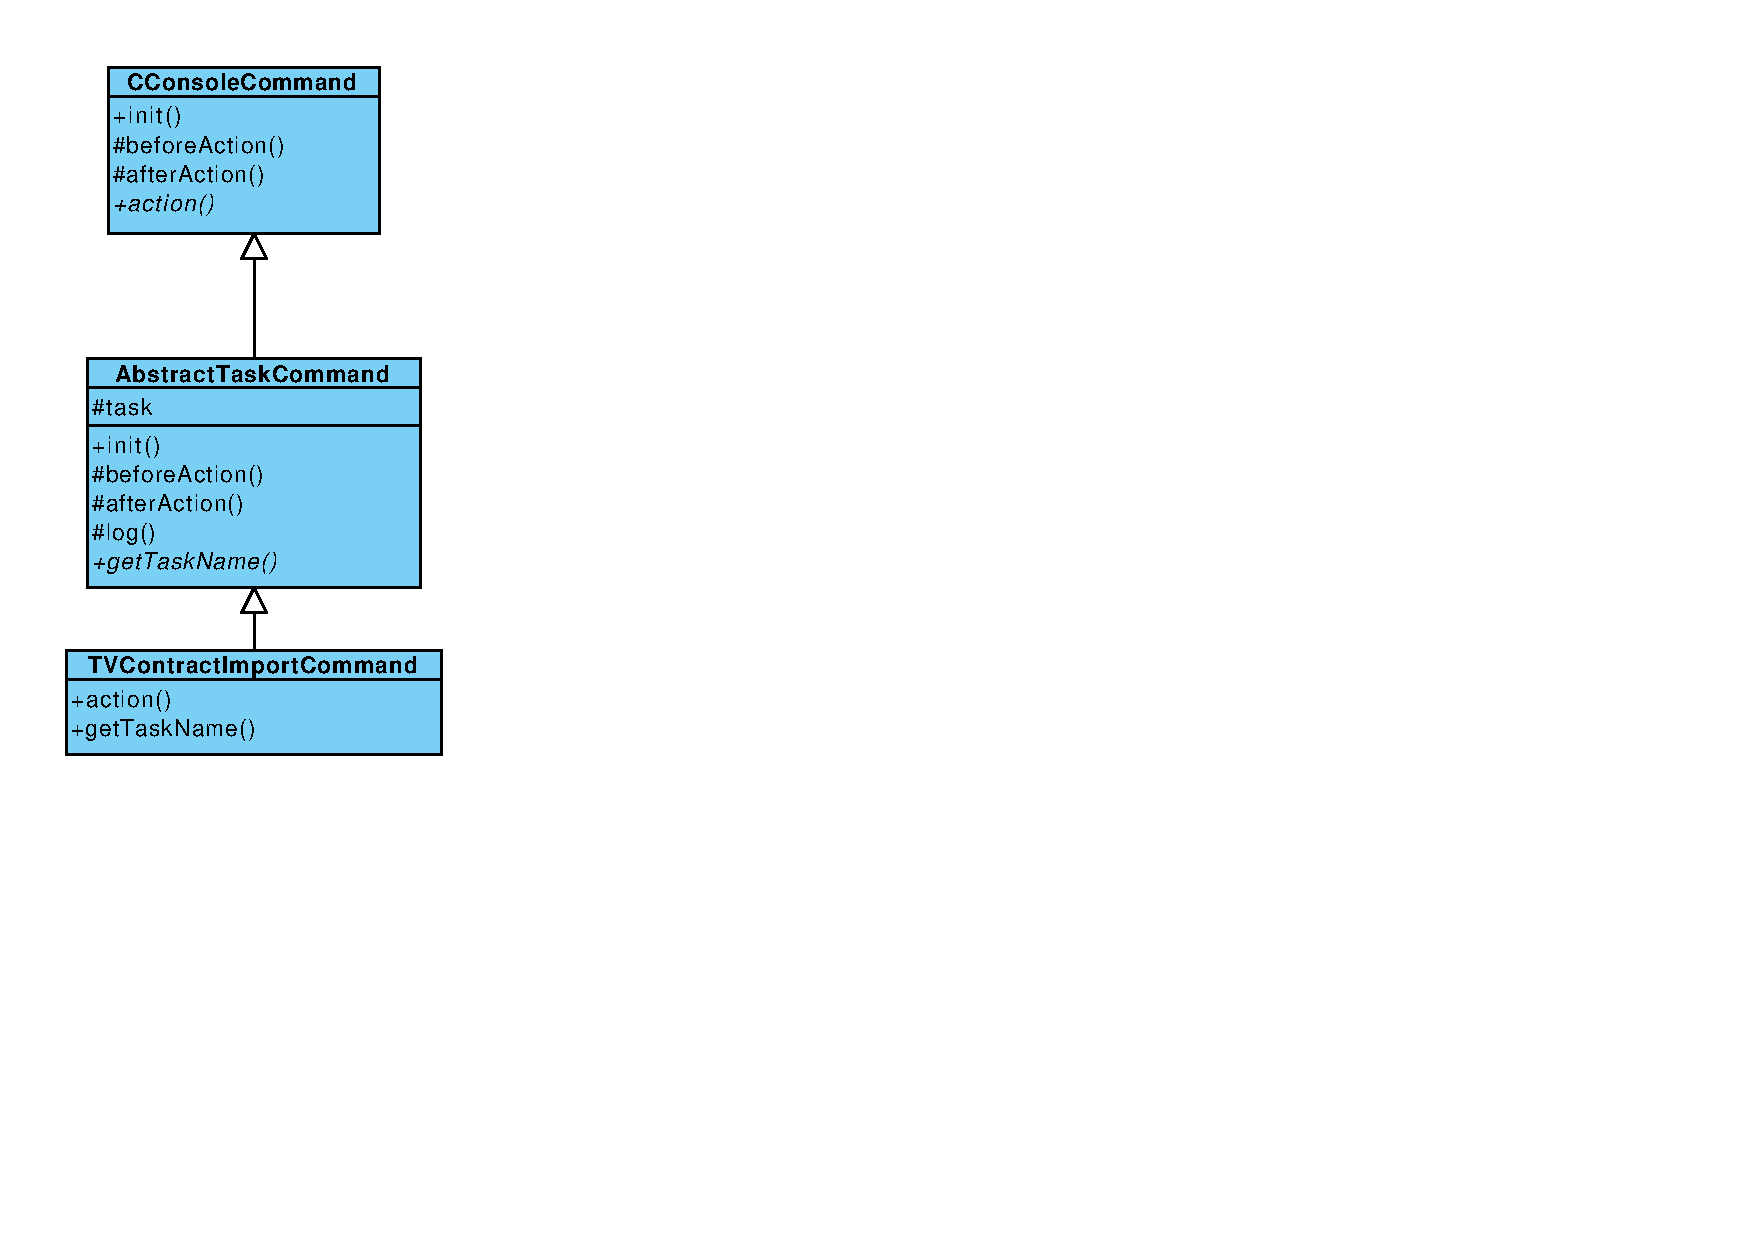
\includegraphics[scale=0.7, trim=10mm 81mm 200mm 10mm, clip]{../resources/uml/AbstractTask.pdf}
\caption{Диаграмма классов с примером реализации консольной команды ``Импорт договоров''}
\label{gr:tasks_class}
\end{center}
\end{figure} 

Описанное решение проблемы запуска фоновых задач делает такие трудоемкие операции, как построение отчетов
или расчет отчислений, в высокой степени горизонтально масштабируемыми за счет возможности увеличения
числа машин-воркеров.

\subsubsection{Миграции структуры БД}
В процессе разработки веб-приложений, особенно в случае работы команды, возникает проблема
синхронизации схемы базы данных, как в локальных версиях разработчиков, так и на тестовых
и production-серверах.

Для решения этой проблемы в Yii предлагается использовать механизм миграций.
В случае необходимости изменений схемы БД разработчик генерирует шаблон миграции с помощью 
консольной команды:

\textit{yiic migrate create <migration-name>}.

Шаблон миграции представляет собой класс, имя которого состоит из timestamp времени генерации
и выбранного имени миграции. В классе определены два пустых метода: \textit{up()} и \textit{down()}.
В первом из них определяется список SQL команд, которые следует выполнять для применения новой схемы,
второй содержит команды, возвращающие состояние схемы в исходное состояние.

Для определения состояния схемы в настоящий момент времени используется служебная таблица
``tbl\_migration'', в которой хранится список примененных миграций и время применения.
При получении обновлений из системы контроля версий или при обновлении на сервере
разработчик может запустить команду 

\textit{yiic migrate}, 

в результате работы которой применятся все новые миграции в том порядке,
в котором они были добавлены разработчиками. Причем в большинстве случаев изменения происходят
без потери существующих данных.

При применении миграций не могут быть исключены ошибки исполнения SQL-комманд,
связанные с разным набором данных на серверах. В этом случае применение миграций останавливается,
и пользователю выводится соответствующее уведомление об ошибке. В связи с ограничением доступа
к системе в режиме production, ее обновление будет производиться заказчиком самостоятельно,
таким образом в случае возникновения ошибок миграции вероятней всего придется добавлять в систему
новые миграции, причем желательно, чтобы уже запущенная миграция в итоге применилась без ошибок.

Для этого в рамках разработки системы было решено не использовать миграции, состоящие из нескольких
SQL-команд, чтобы не возникало ситуации, когда запущенная миграция завершается с ошибкой, выполнив 
при этом часть команд.

\subsubsection{Диаграмма развертывания}
\begin{figure}[!ht]
\begin{center}
\vspace{-0.5cm}
\includegraphics[scale=0.6, trim=10mm 50mm 0mm 10mm, clip]{../resources/uml/Deployment.pdf}
\caption{Схематичная диаграмма развертывания системы}
\label{gr:deployment}
\end{center}
\end{figure} 

Из диаграммы развертывания системы (рис. \ref{gr:deployment}) видно, что в качестве веб-сервера
системы предлагается к использованию Apache, который соединен с приложением с помощью модуля \textit{mod\_php}.
Веб-приложение Reports соединяется с СУБД Microsoft SQL Server 2008, находящейся на выделенном
сервере под управлением операционной системы Windows Server 2003, посредством протокола ODBC.
Сервер очередей задач Gearman располагается на том же хосте, что и веб-приложение, а экземпляры-воркеры
могут быть запущены на отдельном сервере, имеющем сетевой доступ, как к основному серверу,
так и к серверу СУБД.
